\documentclass[../NormediProgetto.tex]{subfiles}

\begin{document}
	
	\chapter{Processi Organizzativi}
	
	\section{Scopo}
	Lo scopo di questo processo è fornire norme e strumenti per organizzare il lavoro del gruppo per il corretto svolgimento del progetto.
	
	\section {Descrizione}
	Durante questo processo sono trattati:
	\begin{itemize}
		\item Ruoli di progetto;
		\item Comunicazioni;
		\item Incontri;
		\item Strumenti di coordinamento;
		\item Strumenti di versionamento.
		
	\end{itemize}
	
	\section {Ruoli di progetto}
	
	Ogni ruolo viene ricoperto da ciascun componente del gruppo a turno, dando la possibilità ad ogni membro di fare esperienza in ognuno di essi. L'organizzazione e la pianificazione delle attività da svolgere in ogni ruolo è regolata dal PP. La descrizione dei ruoli viene approfondita nelle sezioni seguenti.
	
	\subsection {Amministratore di Progetto}
	
	L’\textit{Amministratore di Progetto} deve controllare e amministrare tutto l’ambiente di lavoro con piena responsabilità sulla capacità operativa e sull’efficienza. 
	\\ \noindent Le sue mansioni sono: 
	
	\begin{itemize}
		\item ricerca di strumenti che migliorino l’ambiente di lavoro e che lo automatizzino ove possibile;
		\item gestione del versionamento;
		\item controllo di versioni e configurazioni del prodotto software; 
		\item risoluzione dei problemi di gestione dei processi; 
		\item controllo della \glossario{qualità}{qualita} sul prodotto.
	\end{itemize}
	
	\subsection {Responsabile di Progetto}
	
	Il \textit{Responsabile di Progetto} è il punto di riferimento sia per il \glossario{committente}{committente} che per il \textit{fornitore}. Esso deve anche approvare le scelte prese dal gruppo e se ne assume la responsabilità. 
	\\ \noindent Le sue mansioni sono:
	
	\begin{itemize}
		\item coordinare e pianificare le attività di progetto;
		\item approvare la documentazione;
		\item effettuare uno studio e gestire in modo corretto i rischi;
		\item approvare l'offerta economica;
		\item gestire le risorse umane distribuendo in modo corretto i carichi di lavoro.
	\end{itemize}
	
	\subsection {Analista}
	
	L'\textit{Analista} si occupa dell'analisi dei problemi e del dominio applicativo. Normalmente questo ruolo non rimane attivo per tutta la durata del progetto, bensì concentra tutta la propria attività nelle fasi iniziali.
	\\ \noindent Le sue principali mansioni sono:
	
	\begin{itemize}
		\item comprensione del problema e della sua complessità;
		\item produzione dello \textit{Studio di Fattibilità} e dell'\textit{Analisi dei Requisiti}.
	\end{itemize}
	
	\subsection {Progettista}
	
	Il \textit{Progettista} gestisce gli aspetti tecnologici e tecnici del progetto.
	\\ \noindent Le sue mansioni sono:
	
	\begin{itemize}
		\item rendere facilmente mantenibile il progetto;
		\item effettuare scelte efficienti ed ottimizzate su aspetti tecnici del progetto.
	\end{itemize}
	
	\subsection {Verificatore}
	
	Il \textit{Verificatore} deve garantire una verifica completa ed esaustiva del progetto basandosi sulle solide conoscenze delle sue normative.
	\\ \noindent Le sue mansioni sono:
	\begin{itemize}
		\item controllare le attività del progetto secondo le normative prestabilite.
	\end{itemize}
	
	\subsection {Programmatore}
	
	Il \textit{Programmatore} è il responsabile della codifica del progetto e delle componenti di supporto, che serviranno per effettuare le prove di verifica e validazione sul prodotto.
	\\ \noindent Le sue mansioni sono:
	
	\begin{itemize}
		\item versionamento del codice prodotto;
		\item implementare le decisioni del \textit{Progettista};
		\item realizzazione degli strumenti per la verifica e la validazione del software;
		\item scrittura di un codice pulito e facile da mantenere, che rispetti le \textit{Norme di Progetto}.
	\end{itemize}
	
	\section{Gestione di progetto}
	
	La gestione di progetto viene effettuata tramite meccanismo di ticketing, di seguito illustrato.
	
	\subsection{Pianificazione tramite ticketing}
	
	All'inizio di ogni incremento il \textit{Responsabile di Progetto} è tenuto a pianificare un insieme di task da assegnare ai componenti del gruppo sulla base di:
	 
	\begin{itemize}
	 	\item una stima delle risorse disponibili per suddetto incremento;
	 	\item una stima dei possibili rischi;
	 	\item rispetto degli obiettivi di qualità definiti.
	\end{itemize}
	 
	\noindent Per l'assegnazione del carico di lavoro in Task equamente distribuiti tra i componenti viene utilizzata la piattaforma \glossario{Wrike}{Wrike}, che mostra in modo efficace nella propria interfaccia il quadro completo di tutti i Task inseriti con relativo status (completato, in corso o libero), persona assegnata e scadenza. Quando viene inserito, viene assegnato o cambia stato un Task viene inviata una mail ad ogni componente del gruppo e, per tutti i componenti che fanno uso dell'applicazione mobile, viene inviata una notifica sugli smartphone collegati a \textit{Wrike}.
	\\ \noindent L'assegnazione dei Task avviene secondo il seguente schema:
	
	\begin{itemize}
		\item inserire un titolo al Task;
		\item dividere in più Subtask il Task e titolarli;
		\item indicare la persona a cui è stato assegnato ogni Subtask;
		\item inserire la data entro cui consegnare i documenti/file nella repository prefissata;
		\item inserire una descrizione che contiene un breve riassunto del compito assegnato e il ruolo assunto in quella fase del progetto.
	\end{itemize}
	
	Segue il diagramma di flusso che riassume la procedura di individuazione e assegnazione dei task:
	
	\begin{figure}[H]
		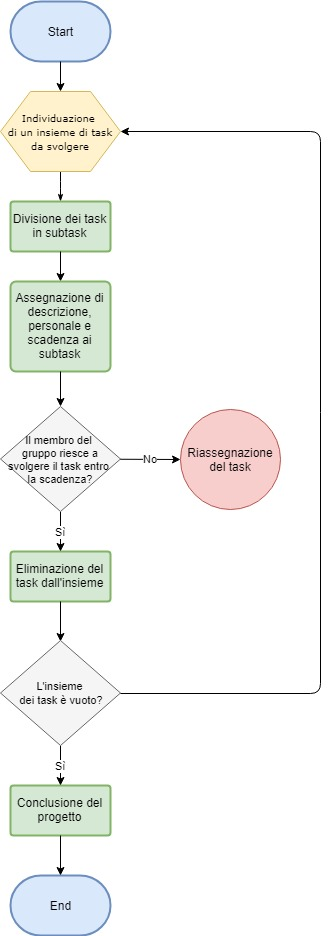
\includegraphics[scale=0.6]{ticketing}
		\centering
		\caption{Diagramma della procedura di individuazione e assegnazione dei task}
	\end{figure}
	
	\subsection{Gestione delle comunicazioni}
	
	\subsubsection{Comunicazioni interne}
	
	Le comunicazioni interne avvengono tramite un tool di messaggistica multi-piattaforma di nome \glossario{Slack}{Slack} con funzionalità specifiche per gruppi di lavoro. Tale strumento offre la possibilità di ricevere notifiche riguardanti le modifiche della \glossario{repository}{Repository} \glossario{GitHub}{GitHub}, creare canali tematici per rendere più efficiente lo scambio e il reperimento delle informazioni, condividere file ed immagini utili allo sviluppo del progetto.
	\\ \noindent Per comunicazioni informali e per ricevere notifiche riguardanti le modifiche della \glossario{repository}{Repository} \glossario{GitHub}{GitHub} verrà usato un ulteriore tool di messaggistica di nome \glossario{Telegram}{Telegram}.
	\\ \noindent Per mantenere sotto continuo controllo l'avanzamento dei lavori è prevista, almeno una volta a settimana, una conversazione su \textit{Slack} in cui ogni membro del gruppo indica lo stato di avanzamento del \glossario{Task}{task} assegnatogli.
	
	\subsubsection{Comunicazioni esterne}
	
	Il \textit{Responsabile del Progetto} è tenuto a mantenere le comunicazioni esterne utilizzando una cartella di posta elettronica appositamente creata:
	\[graphite.swe@gmail.com.\]
	Il \textit{Responsabile del Progetto} deve mantenere informati i restanti componenti del gruppo riguardo alle discussioni con terzi utilizzando i canali di comunicazione interna. 
	\\ \noindent In ogni caso per evitare disguidi interni è previsto che alla ricezione di una mail sull'indirizzo di posta elettronica il messaggio venga inoltrato a tutti i componenti del gruppo.
	
	\subsection{Gestione degli incontri}
	
	\subsubsection{Incontri interni}
	
	Il \textit{Responsabile di progetto} è incaricato di organizzare gli incontri interni dando comunicazione di data e ora tramite i canali di comunicazione. Inoltre deve essere comunicato prima di ogni riunione l'ordine del giorno sempre dal \textit{Responsabile di progetto}.
	\\ \noindent Per mantenere sotto continuo controllo l'avanzamento dei lavori è previsto almeno un incontro settimanale con l'intero gruppo.
	\\ \noindent Ogni componente del gruppo ha diritto di presentare una richiesta di organizzazione di un incontro al \textit{Responsabile di progetto} il quale può accogliere o meno la proposta.
	
	\subsubsection{Incontri Esterni}
	
	Il \textit{Responsabile di Progetto} deve organizzare gli incontri esterni con il committente e comunicare al proprio gruppo data e ora in cui essi avvengono. Come per gli incontri interni, ogni componente del gruppo ha diritto ad una richiesta di organizzazione di un incontro esterno.
	\\ \noindent Per ogni incontro esterno deve essere preventivamente stilata una serie di domande tale da giustificare la richiesta di un appuntamento con il committente.
	
	
	\subsection{Gestione degli strumenti di versionamento}
	
	\subsubsection{Repository}
	
	Per il versionamento e il salvataggio dei file è previsto l'utilizzo di repository su GitHub. L'\textit{Amministratore di Progetto} si deve occupare della creazione dei repository. In seguito l'\textit{Amministratore} inserirà tutti i componenti del gruppo, i quali dovranno essere in possesso di un account personale, come collaboratori.
	\\ \noindent È previsto l'utilizzo di un repository di nome \textit{progettoSWE} suddiviso nel seguente modo:
	
	\begin{itemize}	
		\item \textbf{Documenti:} contiene la documentazione dell'attività di progetto.
		\item \textbf{Prodotto:} contiene i file del prodotto da realizzare.
	\end{itemize}
	
	\subsubsection{Tipi di file e .gitignore}
	
	Nelle cartelle contenenti tutti i documenti saranno presenti solamente i file .tex, .pdf, .jpg, .png. Le estensioni dei file generati automaticamente dalla compilazione sosno stati aggiungi a .gitignore, e quindi vengono ignorati e resi invisibili a \glossario{Git}{Git}.
	
	\subsubsection{Norme sui commit}
	
	Ogni volta che vengono effettuate delle modifiche ai file del repository, le quali poi vengono caricate su di esso, bisogna specificarne le motivazioni. Questo avviene utilizzando il comando \textit{commit} accompagnato da un messaggio riassuntivo e una descrizione in cui va specificato: 
	\begin{itemize}
		\item la lista dei file coinvolti;
		\item la lista delle modifiche effettuate, ordinate per ogni singolo file.
	\end{itemize}

	\subsection{Gestione dei rischi}
	
	Il \textit{Responsabile di Progetto} ha il compito di rilevare i rischi indicati nel PP. Nel caso ne vengano individuati di nuovi dovrà aggiungerli nell'analisi dei rischi dello stesso documento. 
	\\ \noindent La procedura da seguire per la gestione dei rischi è la seguente:
	\begin{itemize}
		\item registrare ogni riscontro dei rischi nel PP;
		\item aggiungere i nuovi rischi individuati nel PP;
		\item individuare problemi non calcolati e monitorare i rischi già previsti;
		\item ridefinire, se necessario, le strategie di progetto.
	\end{itemize}
	
	\section{Strumenti}
	
	\subsection{Organizzazione interna}
	
	\subsubsection{Sistema operativo}
	
	Il gruppo di progetto lavora sui seguenti sistemi operativi:
	\begin{itemize}
		\item Ubuntu 17.10 x64;
		\item Ubuntu 16.04 \glossario{LTS}{LTS} x64;
		\item Windows 10 Home x64;
		\item Windows 10 Pro x64;
		\item Windows 7 Home Premium.
	\end{itemize}
	
	\subsubsection{Slack}
	
	\textit{Slack} è uno strumento di collaborazione aziendale utilizzato particolarmente per lo scambio di messaggi tra componenti di un team. L'idea di partenza di questo software è di essere un totale rimpiazzo degli scambi di E-mail e sms ma a questo si aggiunge la possibilità di aggiungere plugin per la notifica di attività annesse al proprio ambiente di lavoro.
	\\ \noindent Verranno in particolare sfruttati i plugin per la notifica di attività sulla repository e per discussioni riguardo ai task presenti sulla piattaforma Wrike.
	
	\subsubsection{Telegram}
	
	\textit{Telegram} è una applicazione di messaggistica nata come applicazione mobile e successivamente portata anche su Windows, Mac e varie distribuzioni Linux. Rispetto agli altri sistemi di messaggistica \textit{Telegram} consente un facile passaggio di immagini e documenti in più formati mantenendo inoltre nel proprio cloud storage tali file per un agevole recupero su qualsiasi dispositivo. È possibile creare gruppi di utenti la cui chat ha soprattutto il valore aggiunto di poter contenere sistemi automatici per l'organizzazione di sondaggi e la comunicazione di messaggi importanti da tenere in sovraimpressione.
	
	\subsubsection{GitHub}
	
	GitHub è un servizio di \glossario{hosting}{hosting} per progetti software. 
	Il sito è principalmente utilizzato dagli sviluppatori, che caricano il codice sorgente dei loro programmi e lo rendono scaricabile dagli utenti. Può essere utilizzato anche per la condivisione e la modifica di file di testo e documenti revisionabili.
	\\ \noindent Un utente può interagire con lo sviluppatore tramite un sistema di issue tracking, pull request e commenti che permette di migliorare il codice della repository, risolvendo bug o aggiungendo funzionalità.

	\subsubsection{Wrike}

	\textit{Wrike} è un' applicazione web disponibile anche per dispositivi mobile creata per aiutare i team a tracciare il proprio lavoro. Le sue principali funzionalità si dividono in:
	\begin{itemize}
		\item possibilità di creare dei task, assegnarvi delle persone, darne una priorità e controllarne lo stato di completamento;
		\item capacità di creare in modo automatico diagrammi di Gantt basati sui task inseriti dall'utente;
		\item possibilità di condivisione file con la possibilità di farci delle modifiche online;
		\item possibilità di creazione di resoconti e discussioni riguardo a specifici argomenti;
		\item servizio di notifica e modifica rapida tramite l'applicazione per dispositivi mobile.
	\end{itemize}
	Questi servizi sono normalmente disponibili soltanto per la versione a pagamento del software, dando però la possibilità agli studenti di usufruirne con una limitazione di 15 persone per gruppo di lavoro.

	\subsubsection{Git}

	\textit{Git} è un software di controllo versione distribuito utilizzabile da interfaccia a riga di comando. Pensato per mantenere un grande progetto di sviluppo distribuito, Git supporta fortemente lo sviluppo non lineare del software.
	\\ \noindent Tramite strumenti appositi è possibile creare più diramazioni di sviluppo del software con la garanzia di poter mantenere in locale la cronologia di sviluppo completa.
	\\ \noindent In sostituzione ai comandi testuali molti membri del gruppo utilizzeranno \glossario{Gitkraken}{Gitkraken} come interfaccia grafica per la gestione della repository.
	
	% DOCUMENTAZIONE
	
	\subsection{Documentazione}
	
	
	Per redarre la documentazione, il gruppo utilizza i seguenti strumenti:
	
	\begin{itemize}
		\item \textbf{LaTex}: per la stesura della documentazione viene utilizzato il linguaggio \LaTeX{}, data la sua flessibilità, potenza e facilità d'uso;
		
		\item \textbf{TexStudio}: per la stesura del codice \LaTeX{} viene utilizzato l’editor \glossario{TexStudio}{TexStudio}, in virtù delle innumerevoli feature che offre gratuitamente e del fatto che si tratta di un'applicazione cross-platform supportata dai maggiori sistemi operativi;
		
		\item \textbf{SWEgo} Il tracciamento dei requisiti e dei casi d'uso viene effettuato tramite il software \glossario{SWEgo}{SWEgo} e successivamente controllato manualmente per assicurarne la correttezza. Il software è reperibile gratuitamente al link:
		\begin{center}
			\url{http://www.swego.it/}
		\end{center}
		
		\item \textbf{Diagrammi UML}: per la produzione di diagrammi UML viene utilizzato \glossario{Lucidchart}{Lucidchart}. Lo strumento è accessibile al seguenti link: 
		
		\begin{center}
			\centerline{\url{https://www.lucidchart.com/}}
		\end{center}
			
	\end{itemize}

	% SVILUPPO

	\subsection{Sviluppo}

	Per lo sviluppo software relativo al progetto, il gruppo utilizza i seguenti strumenti:

	\subsubsection{IDE}

	Per la codifica relativa al software richiesto dal progetto il gruppo usa l'\glossario{IDE}{IDE} \glossario{Qt}{Qt}, in virtù della sua diffusione, potenza e semplicità d'uso. Qt è reperibile al seguente link:
	
	\begin{center}
		\centerline{\url{https://www.qt.io/}}
	\end{center}

	\subsubsection{Compilazione}

	Per la compilazione vengono utilizzati i seguenti strumenti:

	\begin{itemize}
		\item \textbf{GCC}: il compilatore che verrà usato per la compilazione del software è il \glossario{GCC}{GCC} (GNU Compiler Collection). Il compilatore è reperibile al seguente link:
		
		\begin{center}
			\centerline{\url{https://gcc.gnu.org/}}
		\end{center}
	
		\item \textbf{Cmake}: per semplificare la compilazione verrà usato \glossario{Cmake}{Cmake}. Lo strumento è reperibile al seguente link:
		
		\begin{center}
			\centerline{\url{https://cmake.org/}}
		\end{center}
	
	\end{itemize}

	\subsubsection{GUI}

	Per progettare l'interfaccia grafica viene utilizzato \glossario{Qt Creator}{Qt Creator}. Questo strumento permette di realizzare interfacce grafiche mediante le librerie grafiche Qt, diventate in questo ambito quasi uno standard per piattaforme Linux Based. Qt Creator è disponibile al seguente link: 
	
	\begin{center}
		\centerline{\url{https://www.qt.io/qt-features-libraries-apis-tools-and-ide/}}
	\end{center}
	
	% VERIFICA
	
	\subsection{Verifica}
	
	\subsubsection{Verifica della documentazione}
	
	\begin{itemize}
		\item \textbf{Verifica ortografica:} Per eseguire controlli ortografici sulla documentazione viene utilizzata la verifica dell’ortografia in tempo reale, strumento integrato in TexStudio che sottolinea in rosso le parole errate secondo la lingua italiana;
		
		\item \textbf{Verifica della leggibilità:} Per calcolare l'\glossario{indice Gulpease}{indice Gulpease} a verifica della leggibilità dei documenti viene utilizzato uno script apposito reperibile al link seguente:
		
		\begin{center}
			\centerline{\url{https://github.com/LeafSWE/Leaf/tree/master/Documents/Gulpease}}
		\end{center}
	\end{itemize}
	
	\subsubsection{Verifica del software}
	
	\begin{itemize}
		\item \textbf{Analisi statica:} Per l’analisi statica del codice viene usato il software \glossario{Valgrind}{Valgrind}. La \glossario{suite}{suite} di strumenti Valgrind fornisce numerosi strumenti di \glossario{debugging}{debugging} e di \glossario{profiling}{profiling} che aiutano a rendere i programmi più performanti e più corretti. Il più popolare di questi strumenti è chiamato Memcheck, ed è in grado di rilevare molti errori relativi alla memoria comuni nei programmi C e C++ e che possono causare arresti anomali e comportamenti imprevedibili. Valgrind è accessibile al seguente link: \\ \centerline{\url{http://valgrind.org/}};
		
		\item \textbf{Analisi dinamica:} Per l’esecuzione dei test di analisi dinamica viene usato il software \glossario{SonarQube}{SonarQube}, una piattaforma open source per la gestione della qualità del codice. SonarQube è un’applicazione web che produce report sul codice duplicato, sugli standard di programmazione, i test di unità, il \glossario{code coverage}{code coverage}, la complessità, i bug potenziali, i commenti, la progettazione e l’architettura. SonarQube è accessibile al seguente link: \\ \centerline{\url{https://www.sonarqube.org/}}.
		
		\item \textbf{Metriche legate al software:} Per il controllo delle varie metriche viene utilizzato il software \glossario{Better Code Hub}{Better Code Hub}. Better Code Hub è un servizio di analisi del codice sorgente web-based che controlla il codice per la conformità rispetto a 10 linee guida per l'ingegneria del software e fornisce un \glossario{feedback}{feedback} immediato per capire dove concentrarsi per miglioramenti di qualità. Better Code Hub è accessibile al seguente link:\\ \centerline{\url{https://bettercodehub.com/}}
	\end{itemize}

\end{document}